\section{Evidencias complementarias de gestión de Issues}

Con el objetivo de reforzar la documentación de la práctica, se obtuvieron evidencias adicionales del proceso de administración de incidencias tanto desde la interfaz web de GitHub como mediante GitHub CLI. Estas evidencias permiten observar de forma visual las diferentes acciones realizadas durante el ciclo de vida de un Issue, desde su creación hasta su cierre.

\subsection{Gestión de incidencias mediante GitHub Web}

Después de la creación de la incidencia, se realizó la incorporación de comentarios de seguimiento utilizando la interfaz web de GitHub. Esta funcionalidad permite registrar observaciones, avances y acuerdos relacionados con la incidencia, facilitando la comunicación entre los integrantes del equipo y manteniendo un historial de las actividades realizadas.

\begin{figure}[H]
\centering
\includegraphics[width=0.85\textwidth]{m1.png}
\caption{Registro de comentarios de seguimiento dentro de un Issue mediante GitHub Web.}
\end{figure}

Posteriormente se asignó un responsable para atender la incidencia reportada. La asignación permite identificar claramente al integrante encargado de analizar el problema y dar seguimiento a las acciones necesarias para su resolución.

\begin{figure}[H]
\centering
\includegraphics[width=0.85\textwidth]{m2.png}
\caption{Asignación de un responsable para la atención de la incidencia.}
\end{figure}

Una vez asignado el responsable, se realizaron las actividades necesarias para corregir el problema reportado. El seguimiento del Issue permitió documentar el avance de las tareas hasta alcanzar una solución satisfactoria.

\begin{figure}[H]
\centering
\includegraphics[width=0.85\textwidth]{m3.png}
\caption{Proceso de corrección asociado al Issue reportado.}
\end{figure}

Al concluir la solución del problema, la incidencia fue marcada como resuelta y posteriormente cerrada. Esta acción indica que el trabajo relacionado con el Issue ha finalizado y que no se requieren actividades adicionales.

\begin{figure}[H]
\centering
\includegraphics[width=0.85\textwidth]{m4.png}
\caption{Cierre de la incidencia después de completar la corrección correspondiente.}
\end{figure}

Finalmente se verificó que la incidencia apareciera dentro del listado de Issues cerrados del repositorio. Esta comprobación permitió confirmar que el proceso de gestión se completó correctamente y que toda la información quedó registrada dentro del historial del proyecto.

\begin{figure}[H]
\centering
\includegraphics[width=0.85\textwidth]{m5.png}
\caption{Visualización de incidencias completadas y cerradas dentro del repositorio.}
\end{figure}

\subsection{Validación de operaciones mediante GitHub CLI}

Además de las actividades realizadas desde la interfaz web, se obtuvieron evidencias complementarias relacionadas con la administración de incidencias utilizando GitHub CLI.

Inicialmente se verificó que la incidencia creada desde la terminal hubiera sido registrada correctamente dentro del repositorio. Esta validación permitió comprobar la integración entre GitHub CLI y la plataforma GitHub.

\begin{figure}[H]
\centering
\includegraphics[width=0.85\textwidth]{m6.png}
\caption{Creación de una incidencia utilizando GitHub CLI.}
\end{figure}

Posteriormente se consultó el listado de incidencias disponibles para verificar la aparición del nuevo Issue dentro del repositorio y confirmar que la creación se hubiera realizado correctamente.

\begin{figure}[H]
\centering
\includegraphics[width=0.85\textwidth]{m7.png}
\caption{Verificación del registro correcto de la incidencia creada mediante GitHub CLI.}
\end{figure}

También se visualizaron los detalles completos del Issue, incluyendo información relacionada con su estado, descripción, fecha de creación y demás atributos asociados a la incidencia.

\begin{figure}[H]
\centering
\includegraphics[width=0.85\textwidth]{m8.png}
\caption{Consulta detallada de la información asociada al Issue.}
\end{figure}

Como parte de la administración de incidencias, se asignó un responsable encargado de atender el problema reportado. Esta acción permitió mantener un control adecuado sobre las responsabilidades dentro del proyecto.

\begin{figure}[H]
\centering
\includegraphics[width=0.85\textwidth]{m9.png}
\caption{Asignación de responsable utilizando comandos de GitHub CLI.}
\end{figure}

Asimismo, se incorporó una etiqueta para clasificar la incidencia de acuerdo con su naturaleza. El uso de etiquetas facilita la organización y el filtrado de Issues dentro de proyectos con múltiples incidencias.

\begin{figure}[H]
\centering
\includegraphics[width=0.85\textwidth]{m10.png}
\caption{Clasificación de la incidencia mediante etiquetas.}
\end{figure}

Posteriormente se registraron comentarios de seguimiento que permitieron documentar el avance de las actividades realizadas para la atención del problema reportado.

\begin{figure}[H]
\centering
\includegraphics[width=0.85\textwidth]{m11.png}
\caption{Comentarios agregados durante el seguimiento de la incidencia.}
\end{figure}

Una vez aplicada la solución correspondiente, se documentó la corrección realizada y se verificó el funcionamiento adecuado del sistema.

\begin{figure}[H]
\centering
\includegraphics[width=0.85\textwidth]{m12.png}
\caption{Evidencia de la corrección realizada sobre la incidencia reportada.}
\end{figure}

Finalmente se procedió al cierre de la incidencia y se verificó que ésta apareciera dentro del conjunto de Issues completados, confirmando la finalización satisfactoria del proceso de gestión.

\begin{figure}[H]
\centering
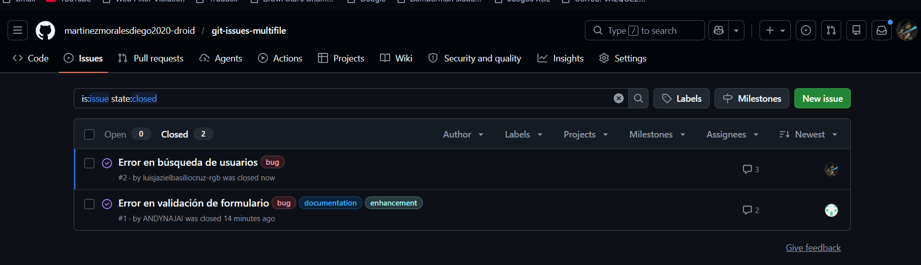
\includegraphics[width=0.85\textwidth]{image.png}
\caption{Listado final de incidencias cerradas después de concluir el proceso de seguimiento y resolución.}
\end{figure}
